\documentclass{article}
\usepackage[english,russian]{babel}
\usepackage{graphicx}
\usepackage{hyperref}
\usepackage{multicol}
\usepackage{indentfirst}
\usepackage[left=1cm,right=1cm,
    top=1cm,bottom=1cm,bindingoffset=1cm]{geometry}
\graphicspath{ {./images/} }
\begin{document}
\selectlanguage{english}
\setlength\parindent{1.5em}
\twocolumn{
 \begin{figure}
     \centering
     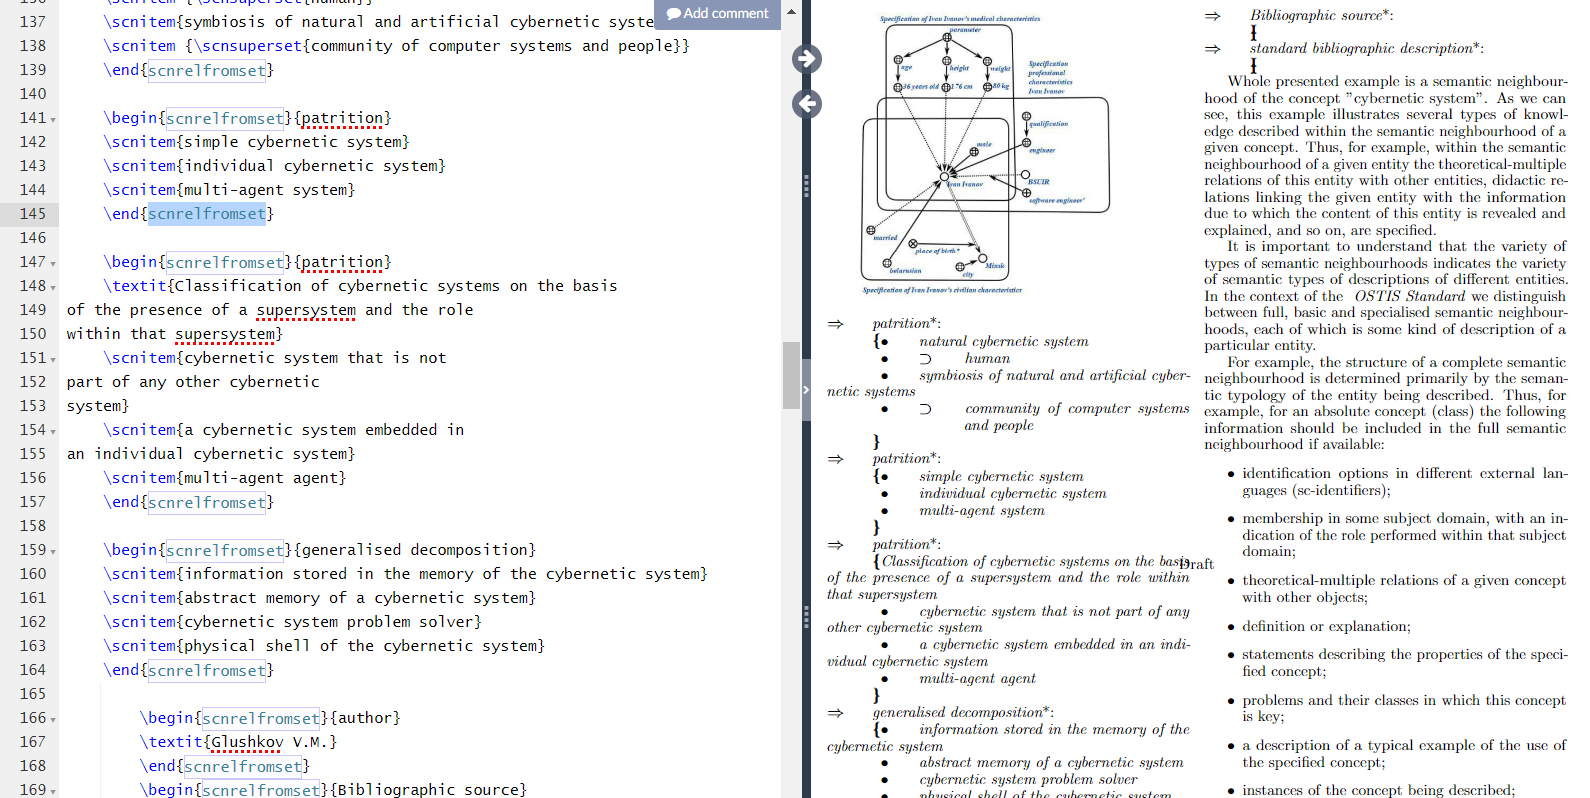
\includegraphics[width=0.85\linewidth]{image.png}
     \caption{ Objects detected after model training}
 \end{figure}
\centering\subsection*{V. Conclusion}
\raggedright 
\hspace{4mm}This paper proposes a concept for the development of robotic ostis-systems. The proposed approach is based on the integration of robotic, symbolic and neural network components in a single system. The application of OSTIS technology for building intelligent robotic systems is sub-stantiated, and the formalization of this subject domain is performed. Practical advice on the development of robotic ostis-systems is given.\par
\hspace{4mm}Areas for future work include:
\begin{itemize}
    \item increasing the versatility of the proposed concept
by expanding the range of described types of robots
and other auxiliary devices;
\item finalization of the existing prototype system for
implementation in production processes;
 \item implementation of diagnostic agents for the system
components;
\item finalization of the agents for calculation of the
mani-pulator trajectory for arbitrary object position.
\end{itemize}
\center\begin{thebibliography}{}
  {\raggedright\footnotesize
  \bibitem{} {M. Thosar, S. Zug, A. M. Skaria, and A. Jain, “A review of
knowledge bases for service robots in household environments,”
in International Workshop on Artificial Intelligence and
Cognition, 2018. [Online]. Available: \href{https://api.semanticscholar.
org/CorpusID:198963468}{https://api.semanticscholar.
org/CorpusID:198963468}
 \bibitem{} D. B. Lenat, “Cyc: A large-scale investment in knowledge infrastructure,” Communications of the ACM, vol. 38, no. 11, pp. 33–38,
1995.
\bibitem{} I. Niles and A. Pease, “Towards a standard upper ontology,” in
Proceedings of the International Conference on Formal Ontology
in Information Systems - Volume 2001, ser. FOIS ’01. New
York, NY, USA: Association for Computing Machinery, 2001, p.
2–9. [Online]. Available: \href{https://doi.org/10.1145/505168.505170}{https://doi.org/10.1145/505168.505170}
\bibitem{} M. Tenorth, D. Jain, and M. Beetz, “Knowledge processing for
cognitive robots,” KI, vol. 24, pp. 233–240, 09 2010.
\bibitem{} M. Tenorth and M. Beetz, “Representations for robot knowledge
in the knowrob framework,” Artificial Intelligence, vol. 247, no. C,
pp. 151–169, 2017.
\bibitem{} V. Golenkov, N. Guliakina, and D. Shunkevich, Otkrytaja
tehnologija ontologicheskogo proektirovanija, proizvodstva
i jekspluatacii semanticheski sovmestimyh gibridnyh
intellektual’nyh komp’juternyh sistem [Open technology of
ontological design, production and operation of semantically
compatible hybrid intelligent computer systems], V. Golenkov,
Ed. Minsk: Bestprint [Bestprint], 2021, in Russ.
\bibitem{} “Raspberry Pi Datasheets,” mode of access : \href{https://datasheets.
raspberrypi.com.}{https://datasheets.
raspberrypi.com} – Date of access : 01.04.2024.
\bibitem{} “HC-SR04-Ultrasonic.pdf,” mode of access : \href{https://www.
handsontec.com/dataspecs/HC-SR04-Ultrasonic.pdf.}{https://www.
handsontec.com/dataspecs/HC-SR04-Ultrasonic.pdf} – Date of
access : 01.04.2024.
\bibitem{} V. Golenkov, Ed., Tehnologija kompleksnoj podderzhki
zhiznennogo cikla semanticheski sovmestimyh intellektual’nyh
komp’juternyh sistem novogo pokolenija [Technology of complex
life cycle support of semantically compatible intelligent computer
systems of new generation ]. Bestprint, 2023, in Russ.
\bibitem{} D. Shunkevich, “Agent-oriented models, method and tools of
compatible problem solvers development for intelligent systems,” Otkrytye semanticheskie tehnologii proektirovanija intellektual’nyh sistem [Open semantic technologies for intelligent systems], pp. 119–132, 2018.
\bibitem{} C.-Y. Wang, A. Bochkovskiy, and H.-Y. M. Liao, “Yolov7: Trainable bag-of-freebies sets new state-of-the-art for real-time object
detectors,” 2022.}}
\end{thebibliography}
\selectlanguage{russian}
{\centering\subsection*{ПРИНЦИПЫ ПОСТРОЕНИЯ
ИНТЕЛЛЕКТУАЛЬНЫХ
РОБОТОТЕХНИЧЕСКИХ СИСТЕМ}}
{{\centering\large\subsection*\textbf{{Крощенко А. А., Ковалёв М. В.}}}\par
\raggedright{ \hspace{4mm} В статье предлагается концепция к построению робототехнических систем коллаборативного типа с использованием технологии OSTIS. Разработанная концепция базируется на интеграции робототехнического, символического и нейросетевого компонентов. Основные положения подхода проиллюстрированы проектом робототехнической системы для сортировки предметов с заданными характеристиками. Даются рекомендации о применении предлагаемой концепции для построения робототехнических систем коллаборативного типа в контексте разработки интеллектуальных компьютерных систем нового поколения, основывающихся на использовании технологии OSTIS.}
\selectlanguage{english}\\
\begin{flushright}
Received 07.04.2024
\end{flushright}
\setcounter{page}{102}
\newpage
\onecolumn
{\centering\section*{ \Huge Methodology of Machine Learning Model
\\Development for Solving Applied Computer
\\Vision Problems}}
\begin{center}
 Marina Lukashevich \par
Information Management Systems Department \par
Belarusian State University \par
Minsk, Belarus \par
\href{LukashevichMM@bsu.by}{LukashevichMM@bsu.by}
\end{center}
\begin{multicols}
\raggedright{
\hspace{4mm}
\textbf{\textit{Abstract}—The methodology of machine learning model development for solving applied computer vision problems is presented. The article discusses the tasks of computer vision, the main components of building application systems and the challenges and limitations of the existing technological level.
\\\hspace{4mm} \textit{Keywords}—Machine learning, computer vision, machine learning model, image, video}
{\subsection*{I. Introduction}}
\hspace{4mm}Machine learning (ML) is the creation and application of models internalized from data. In the case of traditional programming, rules are expressed in a programming language. They act on data, and computer programs provide answers. In the case of machine learning, the answers (typically called labels) are provided along with the data, and the machine infers the rules that determine the relationship between the answers and the data. Machine learning involves algorithms that learn from patterns of data and then apply them to decision making (Figure 1).}
\begin{fi}
        \includegraphics[width=0.9\linewidth]{095143.jpg}
        \caption{Figure 1. Machine learning vs. traditional programming}
    \end{fi}
    \newline
\\\hspace{4mm}Machine learning can also be defined as the process of solving a practical problem by:
\begin{itemize}
    \item collecting a dataset;
    \item algorithmically training a statistical model on that dataset.
\end{itemize}
\hspace{4mm}Machine learning does not have a clear sequence of steps because it is necessary to work with different types of data (tabular data, images, video, signals, text, speech, etc.) and in different domains (data analysis, computer vision, natural language processing, robotics, etc.). Each case has its own specifics, algorithmic techniques, and tools. The main goal of this paper is to summarize theoretical background and practical experience, formalize a methodology for machine learning model building for solving computer vision problems, and formulate some practical recommendations.
\subsection*{II. Computer vision analysis}
   \subsubsection*{ \textit{A. Computer vision}}
    \hspace{4mm}Computer vision (CV) is defined as the automatic extraction of information from images or videos. Sometasks require computer vision to simulate human vision. In other cases, it is necessary to perform statistical data processing, geometric transformations, etc. In practice, computer vision is a fusion of artificial intelligence, pattern recognition, digital signal and image processing, math, and physics (Figure 2). It depends on the specific problem being solved. \par   
    \begin{fi}
        \includegraphics[width=0.9\linewidth]{100402.jpg}
        \caption{Figure 2. Interdisciplinarity of computer vision}
        \label{fig:enter-label}
    \end{fi}
    \setcounter{page}{103}
\newpage
\center\subsubsection*{\textit{ B. Object and scene level tasks}}
\begin{flushleft}\hspace{4mm}The focus of object-level tasks is on objects in a visual scenario, and they require the analysis and understanding of various entities or instances that are associated with them. These tasks involve recognizing objects, detecting them, tracking them, detecting changes, detecting anomalies, and segmenting them. 
\\\hspace{4mm}The process of object recognition involves identifying and categorizing objects into predetermined classes or categories. In object detection, the procedure of recognizing and precisely locating an object within an image or video is performed by creating a bounding box around it. \\\hspace{4mm}The process of tracking the movement of objects across multiple frames of aerial video or image sequences is referred to as object tracking. \\\hspace{4mm}The process of identifying alterations in imagery over different time instances is called change detection. The process of systematic identification of abnormal patterns or objects within visual data and contrasting them with established norms is referred to as anomaly detection. 
\\\hspace{4mm}In semantic segmentation, semantic labels or classes are assigned to each pixel in an image. In the case of instance segmentation, semantic labels, or class labels, are assigned to each pixel in an image with distinction between individual instances of the same class. The complexity and list of computer vision tasks for object level are presented in Figure 3. \\\hspace{4mm}Scene-level tasks focus on a specific scene or an entire image or video scenario in visual data and involve indepth analysis of context, composition, or environmental features. Tasks such as image registration, 3D reconstruction and terrain modeling, and localization and mapping are some of the scene-level tasks. The complexity and list of computer vision tasks for scene level are presented in Figure 4.\end{flushleft}
\subsubsection*{\textit{C. Revolution in computer vision}}
\center\begin{raggedright}\hspace{4mm}In 2006, Nvidia released CUDA, a programming language that allowed GPUs to be used as generalpurpose supercomputers. In 2009, artificial intelligence researchers at Stanford introduced Imagenet, a collection of labeled images used to train computer vision algorithms. A revolution in computer vision occurred when neural networks aimed at working with images began to be used. These are called convolutional neural networks. In 2012, convolutional neural networks (AlexNet) significantly reduced the error in classification and approached the result, which shows in image recognition by a human about 5\% of errors. And in 2015, neural networks overtook humans in recognition accuracy and showed a result of 3.6\%. CNN, the ImageNet dataset, and graphics processors were the magic combination that launched a powerful advance in computer vision. In the last few years, neural networks based on transformer architecture with Attention mechanism have shown excellent efficiency in computer vision. 
\\\hspace{4mm}The most effective solutions in the field of computer vision are based on neural networks in general and on deep neural networks in particular. A large number of effective architectures of deep neural networks have been proposed by researchers. These architectures are implemented in modern deep learning frameworks and are widely used in practice. The classical theory of pattern recognition and digital image processing began to take a back seat. The classical scheme, including image preprocessing, feature computation, and decisionmaking, has become less effective. The use of neural networks involves feature computation and decision making by the neural network itself [1]–[8].
\subsection*{III. Components for solving computer vision problems}
\hspace{4mm}Highlight the main components necessary for realizing practical solutions for machine learning tasks.\end{raggedright}
\begin{itemize}
    \item Datasets.
\item Frameworks and libraries.
\item Model architecture.
\item Hardware resources.
\end{itemize}
\hspace{4mm}Machine learning models are built on the basis of data. Two types of datasets can be identified:
\begin{itemize}
    \item large datasets used for model pre-training and implementation of transfer learning technology (for example, ImageNet, COCO, etc.);
 \item custom datasets are collected and labeled for a specific task
\end{itemize}
\raggedright
\hspace{4mm}It is a good solution for scientific and educational tasks to use public datasets from well-known platforms (Kaggle, Roboflow, etc.). In addition, it should be mentioned that synthetic data can be used to train models in some cases. Synthetic data can be obtained in the following ways:
\begin{itemize}
    \item using generative neural networks;
\item building 3D models of objects, creating synthetic images and videos with different backgrounds, extraneous objects, etc. on their basis (using Blender, NVidia Omniverse, etc.).
\end{itemize}
\begin{raggedright} 
\hspace{4mm}There are two leading frameworks for deep neural network development: PyTorch and TensorFlow. Both are powerful frameworks with unique strengths. PyTorch is favored for research and dynamic projects, while TensorFlow excels in large-scale and production environments. Industry experts may recommend TensorFlow, while hardcore ML engineers may prefer PyTorch. However, there has been a general trend of increasing usage and preference for Pytorch. 
\\\hspace{4mm}In addition to frameworks, a number of libraries and IDEs are used in building computer vision solutions, as well as in experiments and development processes. Some of them are presented in Table I.
\end{raggedright}
\end{multicols}
\setcounter{page}{104}
\end{document}